After running the DC voltage sweep for the Schottky diode, the following results are measured.

\FloatBarrier

\begin{table}[h!]
	\centering
	\caption{Schottky Diode Results}
	\label{tab:schottky-results}
	\csvautotabular{../tables/schottky_table.csv}
\end{table}

\FloatBarrier

Plotting the currents calculated over the voltages across the diode generates the following figure:

\FloatBarrier

\begin{figure}[h!]
	\centering
	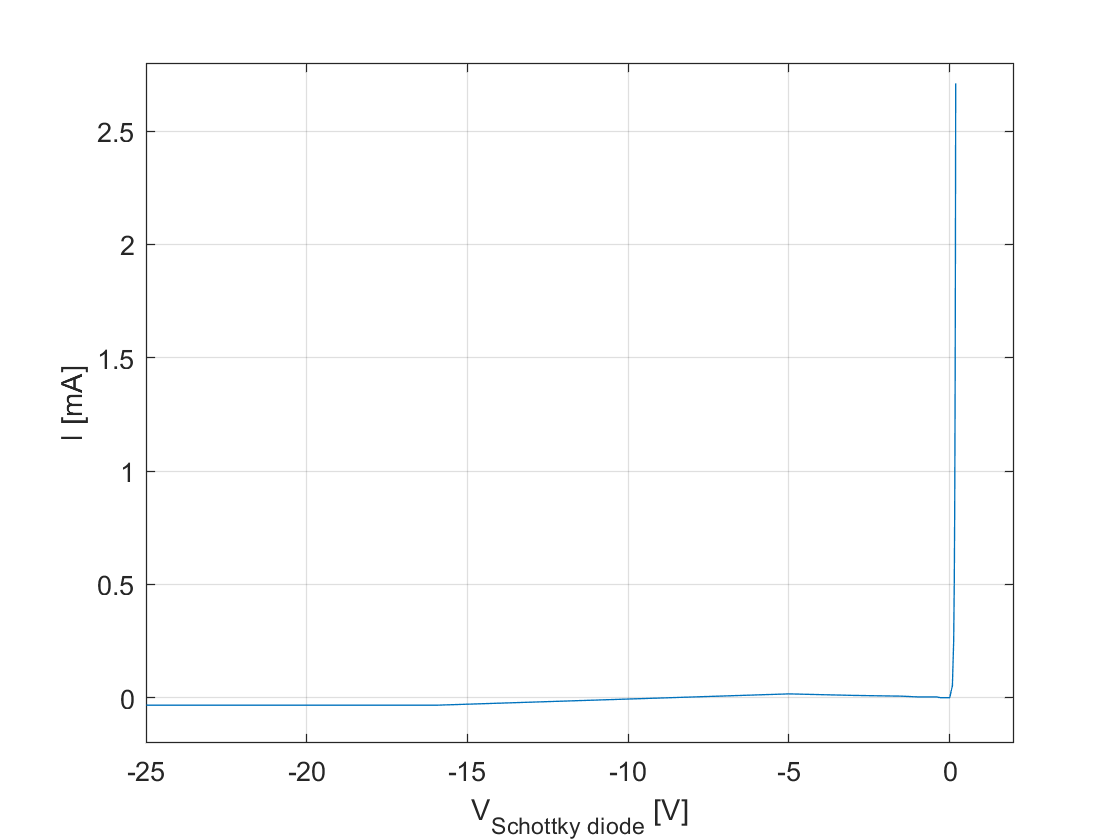
\includegraphics[scale=0.4]{../images/schottky_diode.PNG}
	\caption{Measured IV Characteristic Curve of Schottky Diode}
	\label{fig:schottky_measured}
\end{figure}

\begin{figure}[h!]
	\centering
	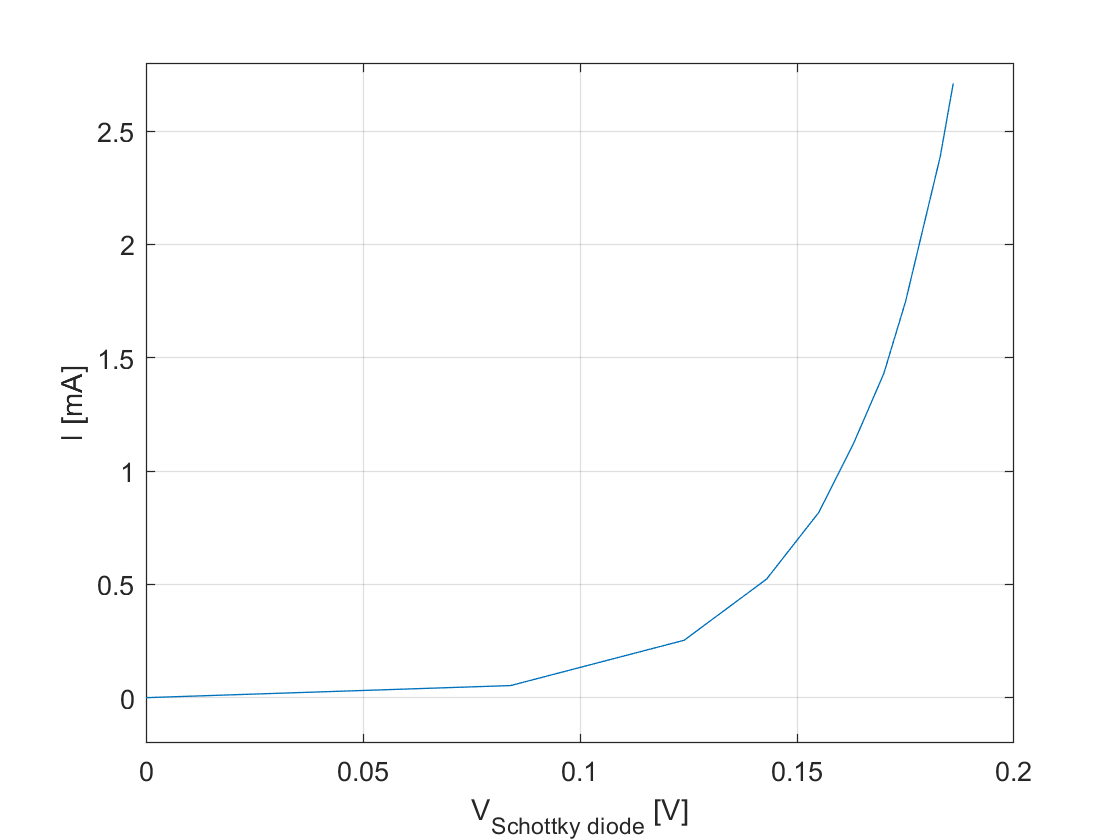
\includegraphics[scale=0.4]{../images/schottky_diode_turn_on.PNG}
	\caption{Measured Turn-on Voltage of Schottky Diode}
	\label{fig:schottky_turn_on}
\end{figure}

\FloatBarrier

Looking more closely at the forward bias portion of the curve (Figure \ref{fig:schottky_turn_on}), the turn-on voltage is observed to be approximately $0.18 V$. Schottky diodes have lower forward turn-on voltages than conventional pn-junction diodes (\ref{ref:schottky_diode_src}), so the observed turn-on voltage is within expectation.

The reverse breakdown voltage of the Schottky diode is again too large to be detected from the DC voltage sweep as seen in Figure \ref{fig:schottky_measured} but the typical values for the breakdown voltage is around $50 V$, considerably lower than the conventional pn-junction diode (\ref{ref:schottky_diode_src}).